\documentclass[t]{beamer}
%\usepackage[orientation=portrait,size=custom,width=8,height=4,scale=0.3,debug]{beamerposter}

\RequirePackage{natbib}
\setcitestyle{authoryear,round,citesep={;},aysep={,},yysep={;}}

\mode<presentation>
{
  \usetheme{default}
  \usecolortheme{default}
  \usefonttheme{professionalfonts}
  \setbeamertemplate{navigation symbols}{}
  \setbeamertemplate{caption}[numbered]
}

\usepackage[english]{babel}
\usepackage[utf8]{inputenc}

\usepackage{amsmath}
\usepackage{amsfonts}
\usepackage{amsthm}
\usepackage{bibentry}
\usepackage{graphicx}
\usepackage{bm}
\usepackage{booktabs}
\usepackage{tikz}
\usepackage{xcolor}
\usepackage{multirow}
\usepackage[normalem]{ulem}
\usepackage{pifont}
\usepackage{array}
\usepackage{multimedia}
\usepackage{makecell}
\usepackage{xspace}
\usepackage{pdfpages}


\renewcommand{\ULthickness}{1.2pt}
%\graphicspath{{../figures/}}
\newcommand{\latexfile}[1]{\input{sections/#1}}
\newcommand{\figfile}[1]{../figures/#1}
\newcommand{\autofig}[1]{../auto_fig/#1}
\newcommand{\datafile}[1]{\input{../data/#1}}

\DeclareMathOperator*{\argmin}{\arg\!\min}
\DeclareMathOperator*{\argmax}{\arg\!\max}

\newcommand{\name}[0]{\abr{clime}} \newcommand{\vect}[1]{\bm{\mathbf{#1}}}
\newcommand{\norm}[1]{\left\lVert#1\right\rVert}



\definecolor{color0}{HTML}{FFFFFF}
\definecolor{color1}{HTML}{FEE5D8}
\definecolor{color2}{HTML}{FDCAB5}
\definecolor{color3}{HTML}{FCAB8F}
\definecolor{color4}{HTML}{FC8A6A}
\definecolor{color5}{HTML}{FB694A}
\definecolor{color6}{HTML}{F14432}
\definecolor{color7}{HTML}{D92523}
\definecolor{color8}{HTML}{BC141A}
\definecolor{color9}{HTML}{980C13}
\definecolor{color10}{HTML}{800080}
\definecolor{easy}{HTML}{02C386}
\definecolor{hard}{HTML}{C00202}
\newcommand*{\mybox}[2]{\tikz[anchor=base,baseline=0pt,rounded corners=0pt,inner sep=0.2mm] \node[fill=#1!60!white] (X) {#2};}
\newcommand*{\mybbox}[2]{\tikz[anchor=base,baseline=0pt,inner sep=0.2mm,] \node[draw=black,thick,fill=#1!60!white] (X) {#2};}


\newcommand{\abr}[1]{\textsc{#1}}
\newcommand{\nlp}{\textsc{nlp}}
\newcommand{\mb}[1]{\boldsymbol{\mathbf{#1}}}
\newcommand{\g}{\, | \,}

\newcommand*\colourcheck[1]{%
  \expandafter\newcommand\csname #1check\endcsname{\textcolor{#1}{\ding{52}}}%
}
\colourcheck{blue}

\title{Interactive Refinement of Cross-Lingual Word Embeddings}
\author{
\tiny{
    Michelle Yuan$^{1*}$ Mozhi Zhang$^{1*}$ Benjamin Van Durme$^2$ Leah Findlater$^3$ Jordan Boyd-Graber$^1$
} \\\vspace{10px}
\tiny{$^1$University of Maryland $^2$John Hopkins University
$^3$University of Washington $^*$Equal contribution}
}
\date{}

\begin{document}



\begin{frame}
    \titlepage
\end{frame}

% authors
%\begin{frame}[c]{Authors}
\begin{center}
\begin{tabular}{ccc}
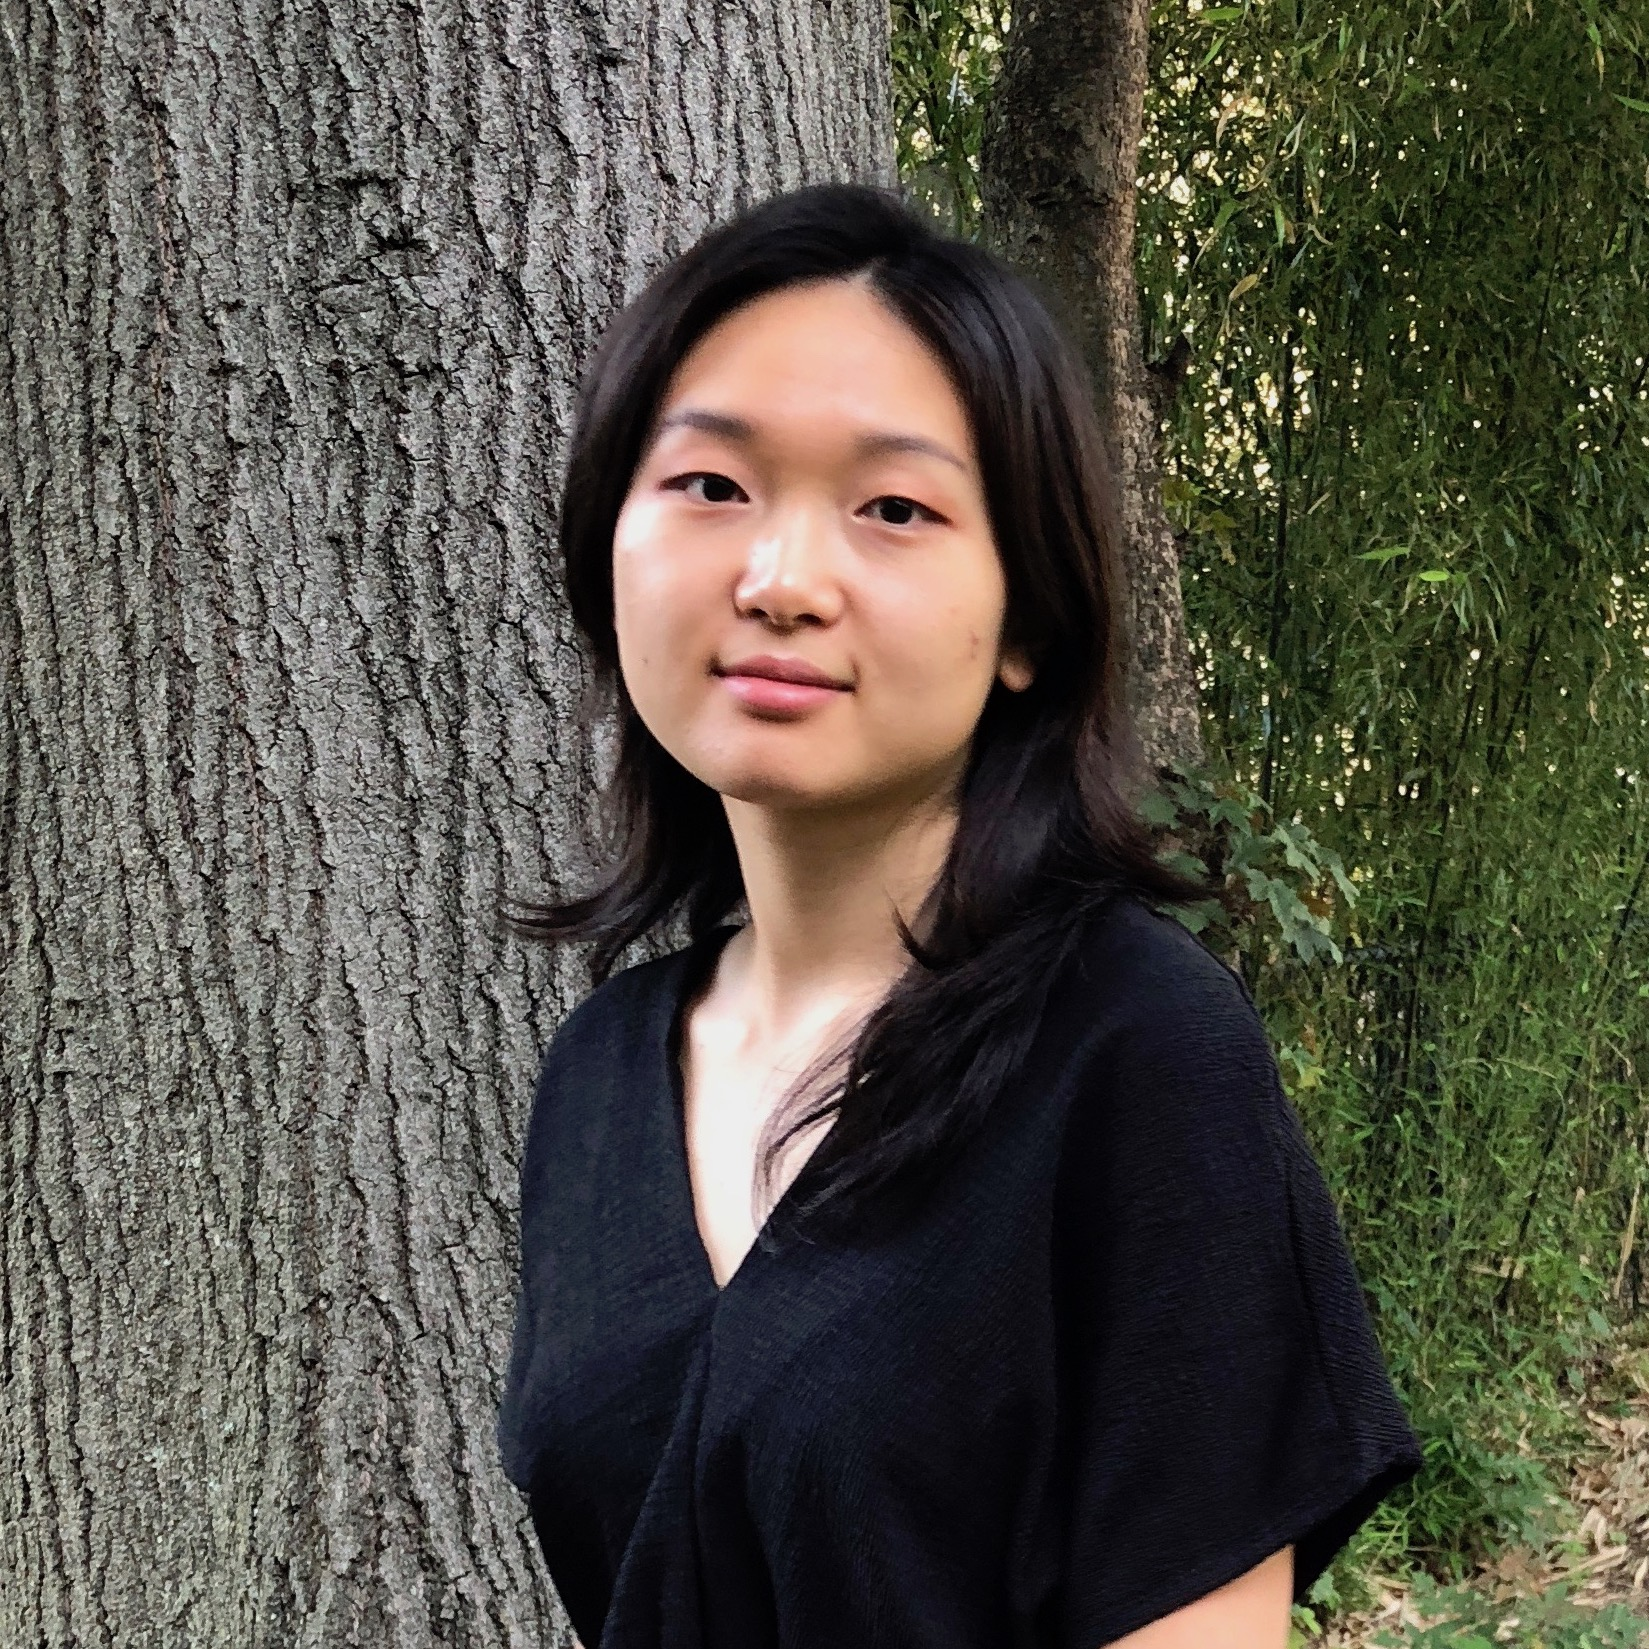
\includegraphics[width=.25\linewidth]{michelle}   & 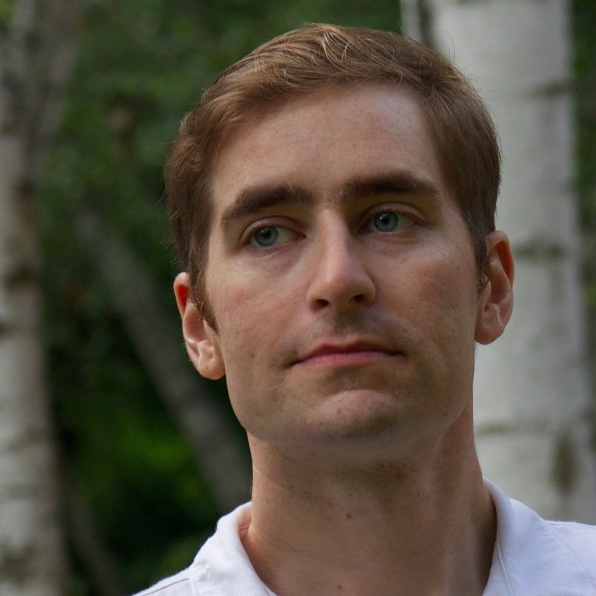
\includegraphics[width=.25\linewidth]{ben}  & 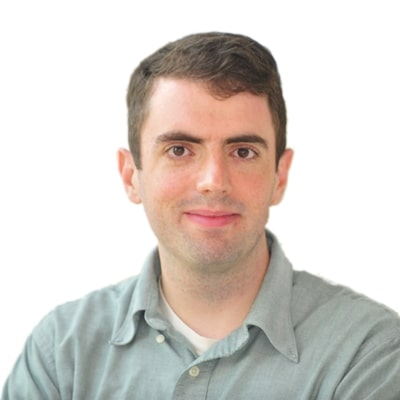
\includegraphics[width=.25\linewidth]{jordan} \\
    Michelle Yuan & Benjamin Van Durme & Jordan Boyd-Graber \\
    UMD & JHU & UMD \\
\end{tabular}
\end{center}
\end{frame}



% 1. clime
\latexfile{10.tex}
% 2. keyword
\latexfile{20.tex}
% % % 3. retrofitting
\latexfile{30.tex}
% % % 4. Experiments
\latexfile{40.tex}
% % % 5. discussion/conclusion
%% conclusion
\begin{frame}{Summary}
\begin{enumerate}
\item Neural CR models cannot immediately adapt without training on in-domain,
labeled data
\item To reduce amount of annotation, we use active learning to choose particular text spans for users to label
\item We explore various aspects of active learning for CR, including sources of
model uncertainty and the trade-off between reading and labeling
\item Sampling by mention detection entropy is more useful for domains like
PreCo
\item In both simulations and the user study,
CR improves from continued training on spans sampled from the same document rather than different
contexts
\end{enumerate}
\end{frame}



\begin{frame}[t, allowframebreaks]
\frametitle{References}
\bibliographystyle{../../style/acl_natbib}
\small
\bibliography{../../bib/journal-abbrv,../../bib/michelle,../../bib/jbg,../../bib/mozhi}
\end{frame}


\end{document}
